% Context budget over a session — 3 stacked horizontal bars showing how
% Fresh / Working / Degraded sessions allocate the finite context window.
%
% Ported from ~/claude-best-practices/chapters/05_context.tex with the
% handbook's locked agent-loop palette substituted:
%   WarmBlue  -> blue   (CLAUDE.md / persistent)
%   WarmGreen -> teal   (task context / working memory)
%   WarmRose  -> orange (noise / threshold annotations)
%   black!5   -> gray!8 (available / free)
%
% Added vs the source: ~83% auto-compaction-trigger annotation (the source
% only shows the ~60% degradation threshold).
\documentclass[tikz,border=4mm]{standalone}
\usepackage{tikz}
\usetikzlibrary{positioning, calc}

\begin{document}
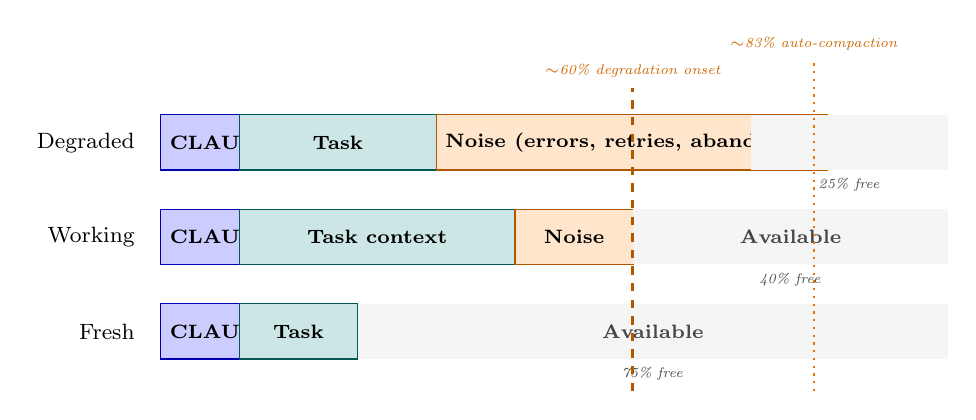
\begin{tikzpicture}[
  font=\sffamily,
  bar/.style={
    minimum height=0.7cm, anchor=south west,
    font=\scriptsize\bfseries, align=center
  },
  lbl/.style={font=\footnotesize, anchor=east},
  pct/.style={font=\tiny\itshape, text=gray!60!black},
  thresh60/.style={dashed, thick, draw=orange!70!black},
  thresh83/.style={dotted, thick, draw=orange!90!black},
  threshlbl/.style={font=\tiny\itshape, text=orange!80!black},
]
  \def\barwidth{10cm}

  % --- Fresh session (~5 min in) ---
  \node[lbl] at (-0.2, 0.35) {Fresh};
  \node[bar, fill=blue!20, draw=blue!70!black, minimum width=0.10*\barwidth] at (0, 0)             {CLAUDE.md};
  \node[bar, fill=teal!20, draw=teal!70!black, minimum width=0.15*\barwidth] at (0.10*\barwidth, 0) {Task};
  \node[bar, fill=gray!8, minimum width=0.75*\barwidth, text=gray!55!black] at (0.25*\barwidth, 0) {Available};
  \node[pct] at (0.625*\barwidth, -0.18) {75\% free};

  % --- Working session (~30 min in) ---
  \node[lbl] at (-0.2, 1.55) {Working};
  \node[bar, fill=blue!20, draw=blue!70!black, minimum width=0.10*\barwidth] at (0, 1.2) {CLAUDE.md};
  \node[bar, fill=teal!20, draw=teal!70!black, minimum width=0.35*\barwidth] at (0.10*\barwidth, 1.2) {Task context};
  \node[bar, fill=orange!20, draw=orange!70!black, minimum width=0.15*\barwidth] at (0.45*\barwidth, 1.2) {Noise};
  \node[bar, fill=gray!8, minimum width=0.40*\barwidth, text=gray!55!black] at (0.60*\barwidth, 1.2) {Available};
  \node[pct] at (0.80*\barwidth, 1.02) {40\% free};

  % --- Degraded session (~90 min in) ---
  \node[lbl] at (-0.2, 2.75) {Degraded};
  \node[bar, fill=blue!20, draw=blue!70!black, minimum width=0.10*\barwidth] at (0, 2.4) {CLAUDE.md};
  \node[bar, fill=teal!20, draw=teal!70!black, minimum width=0.25*\barwidth] at (0.10*\barwidth, 2.4) {Task};
  \node[bar, fill=orange!20, draw=orange!70!black, minimum width=0.40*\barwidth] at (0.35*\barwidth, 2.4) {Noise (errors, retries, abandoned)};
  \node[bar, fill=gray!8, minimum width=0.25*\barwidth, text=gray!55!black] at (0.75*\barwidth, 2.4) {};
  \node[pct] at (0.875*\barwidth, 2.22) {25\% free};

  % --- Threshold annotations ---
  % 60% degradation onset (where quality drops non-linearly)
  \draw[thresh60] (0.60*\barwidth, -0.4) -- (0.60*\barwidth, 3.45)
    node[above, threshlbl] {$\sim$60\% degradation onset};
  % 83% auto-compaction trigger (system-level, stable)
  \draw[thresh83] (0.83*\barwidth, -0.4) -- (0.83*\barwidth, 3.8)
    node[above, threshlbl] {$\sim$83\% auto-compaction};

\end{tikzpicture}
\end{document}
